\documentclass[12pt]{article}
\usepackage[utf8]{inputenc}
\usepackage[top=2.5cm, left=2.3cm, right=2.7cm, bottom=3.0cm]{geometry}
\usepackage{accents}
%\usepackage{amsmath}
\usepackage{float}
\usepackage{hyperref}
\usepackage{pdfpages}
\usepackage{sectsty}
\usepackage{titlesec}
\usepackage{titling}
\usepackage{listings}


\renewcommand{\textbf}[1]{\begingroup\bfseries\mathversion{bold}#1\endgroup}

\title{\textbf{Calcul sécurisé - Contrôle continu} \\ Université de Versailles Saint-Quentin en Yvellines}
\author{SERHAN Wissam 21703993}
\date{Mars 2021}

\begin{document}

    \maketitle
   \vspace{3cm}
    \section*{I/ Attaque par faute sur le 15ème tour}
        \vspace{0.5cm}
        \subsection*{Description détaillée de l'attaque}
        
            \vspace{1cm}
                   \text{
                   Une attaque par faute consiste à l'extraction de données secrétes commme par exemple la clé secréte. L'opération consiste à modifié le comportement habituel de l'algorithme cryptographique par des opération matériels ou logiciels. Dans notre cas, l'attaque par faute aura lieu sur l'algorithme DES par une injection de faute au niveau du $15^{ème}$ tour sur la valeur de sortie $R_{15}$.\\
                   On cherchera donc, par analyse des différences entre le chiffré juste et les chiffrés fautés, à retrouver la clé K16, puis la clé secréte K.\\}
                   \newpage
                   \text{
                   On s'intéressera donc plus particuliéremment au dernier tour de l'algorithme DES :\\}
                   \vspace{1cm}
                   
                   \centerline{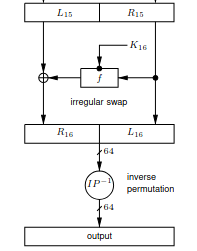
\includegraphics{R15.png}}
                   
                   
                   \text{Pour rappel la faute a lieu au niveau de $R_{15}$. On notera le $R_{15}$ fauté {$\tilde{R_{15}}$}.\\ On obtiendra alors 2 système d'équations :\\} 
                    
                    \paragraph{Sans fautes :}
                    \[\left\{
                      \begin{array}{rcr}
                        R_{16}&=&L_{15}\oplus F(R_{15},K_{16}) \\
                        L_{16}&=&R_{15} \\
                      \end{array}
                    \right.\]
                    \paragraph{Avec fautes :}
                     \[\left\{
                      \begin{array}{rcr}
                        \tilde{R_{16}}&=&L_{15}\oplus F(\tilde{R_{15}},K_{16}) \\
                        L_{16}&=&\tilde{R_{15}} \\
                      \end{array}
                    \right.\]
                    
                    \newpage
                    \underline{\subsubsection*{Description de la fonction $f$ :\\}}\\
                    \centerline{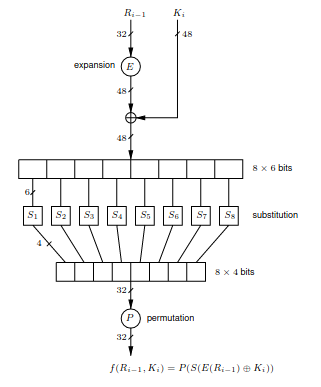
\includegraphics[scale=1.2]{f.png}}
                    \text{En se situant dans le cas précis de $R_{15}$, voici les étapes précises que décrive le schéma :}
                    \vspace{0.5cm}
                    \begin{itemize}
                        \item Initialement de taille 32 bits, $R_{15}$ passe par la fonction d'expansion E et en sort à 48 bits. On note cette étape \textbf{$E(R_{15})$}
                        \item Ensuite, un XOR entre $E(R_{15})$ et la clé $K_{16}$. \\À cette étape nous sommes à \textbf{E(R_{15}) \oplus K_{16}} de taille 48 bits.
                        \item On découpe alors ces 48 bits en 8 paquets de \textbf{6 bits} chacun. Ces 8 paquets vont respectivement passer par leur boite-S correspondantes, notées de $S_1$ à $S_8$, avec une boite-S différente pour chaque paquet. Chaque boite-S prend \textbf{6 bits en entrée} et renvoit \textbf{4 bits en sortie} ce qui redonnera un \textbf{total de 32 bits} comme la taille initiale de $R_{15}$
                        \item Cette sortie de 32 bits va subir une permutation notée \textbf{$P$}.
                    \end{itemize}
                    \newpage
                    \text{
                    De ces différentes étapes on obtient respectivement :\\}
                    \paragraph{Sans fautes :}
                    $$L_{15} \oplus F(R_{15},K_{16}) = L_{15} \oplus P[ S_1( E(R_{15, 1}) \oplus K_{16, 1\rightarrow6}) \parallel S_2( E(R_{15, 2}) \oplus K_{16, 7\rightarrow12}) \parallel ...... \parallel S_8( E(R_{15, 8}) \oplus K_{16, 43\rightarrow48}) ]$$
                    
                    \paragraph{Avec fautes :}
                    $$L_{15} \oplus F(\tilde{R_{15}},K_{16}) = L_{15} \oplus P[ S_1( E(\tilde{R_{15, 1}}) \oplus K_{16, 1\rightarrow6}) \parallel S_2( E(\tilde{R_{15, 2}}) \oplus K_{16, 7\rightarrow12}) \parallel ...... \parallel S_8( E(\tilde{R_{15, 8}}) \oplus K_{16, 43\rightarrow48}) ]$$
                    
                    \text{Or on constate que :}
                    $$R_{16} \oplus \tilde{R_{16}} = F(R_{15},K_{16}) \oplus F(\tilde{R_{15}},K_{16})$$
                    
                    \text{De plus, la fonction de permutation P est inversible car linéaire et que} $$P^{-1}(R_{16} \oplus \tilde{R_{16}}) = P^{-1}(R_{16}) \oplus P^{-1}(\tilde{R_{16}}) $$
                    
                    
                    
                    
                    \textbf{En analysant les différences entre le fauté et en inversant la permutation on obtient : }
                    $$P_{-1} (F(R_{15},K_{16}) \oplus F(\tilde{R_{15}},K_{16})) =$$
                    $$[S_1( E(R_{15, 1}) \oplus K_{16, 1\rightarrow6}) \oplus S_1( E(\tilde{R_{15, 1}}) \oplus K_{16, 1\rightarrow6})] \parallel$$
                    $$[S_2( E(R_{15, 2}) \oplus K_{16, 7\rightarrow12}) \oplus S_2( E(\tilde{R_{15, 2}}) \oplus K_{16, 7\rightarrow12})] \parallel$$
                    $$......$$
                    $$[S_8( E(R_{15, 8}) \oplus K_{16, 43\rightarrow48})\oplus S_8( E(\tilde{R_{15, 8}}) \oplus K_{16, 43\rightarrow48})]$$
                    
                    \text{C'est en découpant cette équation en 8 sous équations correspondants aux 8 S-Box que l'on obtient le système final suivant :}
                    
                    \[\left\{
                      \begin{array}{rcr}
                            P^{-1}(R_{16} \oplus \tilde{R_{16})}_{1\rightarrow6} & = & S_1( E(R_{15, 1}) \oplus K_{16, 1\rightarrow6}) \oplus S_1( E(\tilde{R_{15, 1}}) \oplus K_{16, 1\rightarrow6})\\
                            P^{-1}(R_{16} \oplus \tilde{R_{16})}_{7\rightarrow12} & = & S_2( E(R_{15, 2}) \oplus K_{16, 7\rightarrow12}) \oplus S_2( E(\tilde{R_{15, 2}}) \oplus K_{16, 7\rightarrow12})\\
                            P^{-1}(R_{16} \oplus \tilde{R_{16})}_{13\rightarrow18} & = & S_3( E(R_{15, 3}) \oplus K_{16, 13\rightarrow18}) \oplus S_3( E(\tilde{R_{15, 3}}) \oplus K_{16, 13\rightarrow18})\\
                            P^{-1}(R_{16} \oplus \tilde{R_{16})}_{19\rightarrow24} & = & S_4( E(R_{15, 4}) \oplus K_{16, 19\rightarrow24}) \oplus S_4( E(\tilde{R_{15, 4}}) \oplus K_{16, 19\rightarrow24})\\
                            P^{-1}(R_{16} \oplus \tilde{R_{16})}_{25\rightarrow30} & = & S_5( E(R_{15, 5}) \oplus K_{16, 25\rightarrow30}) \oplus S_5( E(\tilde{R_{15, 5}}) \oplus K_{16, 25\rightarrow30})\\
                            P^{-1}(R_{16} \oplus \tilde{R_{16})}_{31\rightarrow36} & = & S_6( E(R_{15, 6}) \oplus K_{16, 31\rightarrow36}) \oplus S_6( E(\tilde{R_{15, 6}}) \oplus K_{16, 31\rightarrow36})\\
                            P^{-1}(R_{16} \oplus \tilde{R_{16})}_{37\rightarrow42} & = & S_7( E(R_{15, 7}) \oplus K_{16, 37\rightarrow42}) \oplus S_7( E(\tilde{R_{15, 7}}) \oplus K_{16, 37\rightarrow42})\\
                            P^{-1}(R_{16} \oplus \tilde{R_{16})}_{43\rightarrow48} & = & S_8( E(R_{15, 8}) \oplus K_{16, 43\rightarrow48}) \oplus S_8( E(\tilde{R_{15, 8}}) \oplus K_{16, 43\rightarrow48})\\
                      \end{array}
                    \right.\]
                    
                    \text{Afin de retrouver la clé $K_{16}$ on effectue une recherche exhaustive sur les sorties des S-Box : $S_n(E(R_{15}) \oplus K_{16})$.\\
                    Ensuite, pour chaque S-Box on déduits des valeurs d'entrées probables $E(R_{15})\oplus K_{16}$. Dont on en déduit des valeurs $K_{16}$ possibles.}
                    \newpage
                    \text{Pour chaques valeurs de $K_{16}$ possible. On vérifie l'égalité suivante :}
                    $$ P^{-1}(R_{16} \oplus \tilde{R_{16}})_{x\rightarrow y} = S_n( E(R_{15}) \oplus K_{16} )_{x\rightarrow y} $$
                    \text{Si cette égalité est vérifiée, cela signifie que $K_{16, }_{x\rightarrow y}$ devient une portion de clé probable de $K_{16}$. Ainsi pour chacunes des S-Box, on obitendra une clé probables réprésentant respectivement 6 bits de la clé finale $K_{16}$ pour un total de 48 bits. La clé K étant de 56 bits, il conviendra d'inverser les "key schedule" PC1 et PC2 afin d'identifier et de replacer dans un premier temps les 56 bits de la clé secréte $K$ puis d'y ajouter les 8 bits de parité. On retrouve donc bien les 64 bits de la clé secréte.\\}
                    
                    \text{On dispose de 32 chiffrés faux pour lesquels on va effectué la recherche exhaustive des portions de clé de $K_{16}$ et sur les 8 S-Box à chaque fois. On a donc une compléxité totale de l'ordre $O(32\ *\ 2⁶\ *\ 8)\ =\ O(2^{14})$.}
                    
        \subsection*{Mise en oeuvre de l'attaque}
            \text{Pour effectuer cette attaque par faute nous disposons de :}
            \begin{itemize}
                \item 1 chiffré juste
                \item 32 chiffrés faux
            \end{itemize}
            \text{Ces 33 chiffrés découlent d'un seul et même message et d'une seule et même clé.\\
            Il conviendra, comme décris ci-dessus, de retrouver dans un premier temps les 48 bits de la clé $K_{16}$ pour retrouver 48 bits de la clé secréte $K$. Une fois la première question répondue, il conviendra de mener une recherche exhaustive des 8 bits manquants et d'ajouter les bits de parités.\\}
            \text{Pour répondre à ces questions je réaliserais l'implémentation d'un programme en langage C permettant d'automatiser ces tâches en fonctions de chiffrés juste et faux donnés. L'arborescence du projet sera la suivante :\\
            ennoncés/ /* Contenant les énnoncés du contrôle */\\
            README.md\\
            Makefile\\
            chiffre.txt\\
            chiffres\_faux.txt\\
            bin/ /* Contenant les .o */\\
            src/ /* Contenant les .c */\\
            header/ /* Contenant les .h */\\}
            \text{ Pour plus d'informations concernant le code de ce programme : README.md ainsi que les fichier header et src.\\}
            \newpage
            \text{le projet se trouve sur le github : \textcolor{purple}{\url{https://github.com/serwiz/DFA-DES}}\\
            Pour l'utiliser veuillez suivre les instructions indiquée dans le README.md. \\
            Tout les code a été minutieusement expliqué avec des commentaires et les fonctions expliquées.\\Le secret de cette méthode réside dans le ciblage des S-Box, en effet nous disposons d'un grand nombre de chiffré fauté il convient d'identifier le bit mis en cause pour pouvoir analyser l'erreur qui se répend et identifier la S-Box qui en sera affectée. Pour l'identifier il suffit de XOR le fauté avec l'original.}
            
            \text{Le résultat de la console est le suivant :\\\\}
            \vspace{1cm}
            \centerline{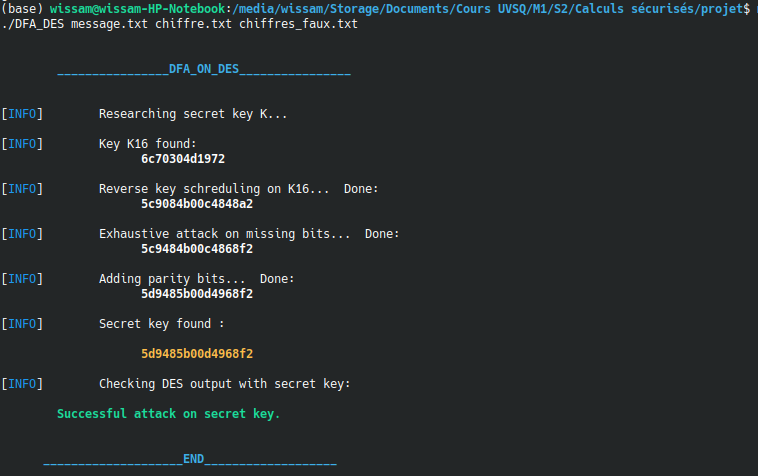
\includegraphics[scale=0.75]{resultat.png}}
            \text{Ainsi, voici les différents résultats concernant la clé K:\\}
            \text{Voici les 48 bits de la sous clé $K_{16}$ :\\ \textbf{\MakeUppercase{$(6c\ 70\ 30\ 4d\ 19\ 72)_{16}$\\$(0110\ 1100\ 0111\ 0000\ 0011\ 0000\ 0100\ 1101\  0001\ 1001\ 0111\ 0010)_{2}$}}\\}
            
            \text{Les 48 bits de la clé $K_{16}$ correspondent a 48 bits de la clé K qu'il faut cependant réorganiser en inversant les PC1 et PC2 tel que $K=PC^{-1}(PC^{-2}(K_{16}))$. Pour remonter à la clé K grâce à la clé $K_{16}$ il faut dans un premier temps inverser les key schreduling PC1 et PC2 on retrouve alors 48 bits de la clé K qui en fait normalement 56 il reste donc 8 bits à trouver. Pour cela il faut mener une recherche exhaustive sur ces bits manquants (très rapide de par sa faible complexité de $2^{14}$). La position de ces bits manquant est connu de tous il manque les bits suivants : \\14, 15, 19, 20, 51, 54, 58, 60\\}
            \text{On se retrouve donc enfin avec les 56 bits de la clé K, il reste donc à ajouter les bits de parité et on aura les 64 bits de la clé K. Ma clé K étant :\\
            \textbf{$(5D\ 94\ 85\ B0\ 0D\ 49\ 68\ F2)_{16}$}}
            
            \text{Pour toutes informations concernant ces étapes merci de vous référer au code celui-ci étant minutieusement expliqué.}
            
    \section*{II/ Attaque par fautes sur les tours précédents}
        
        \text{
        Une attaque par faute sur le $15^{ème}$ tour peut se faire en une complexité de $O(2^{14})$. Mais que ce passe-t-il lorsque l'injection de faute se passe sur le $14^{ème}$ tour par exemple ?\\
        Dans le cas d'une injection de faute sur le $14^{ème}$ tour on se retrouve avec les $R_{15}$ et $L_{15}$ suivants : \\
        \paragraph{Sans fautes :}
                    \[\left\{
                      \begin{array}{rcr}
                        R_{15}&=&L_{14}\oplus F(R_{14},K_{15}) \\
                        L_{15}&=&R_{14} \\
                      \end{array}
                    \right.\]\\
        \paragraph{Avec fautes :}
                    \[\left\{
                      \begin{array}{rcr}
                        \tilde{R_{15}}&=&L_{14}\oplus F(\tilde{R_{14}}, K_{15}) \\
                        L_{15}&=&R_{14} \\
                      \end{array}
                    \right.\]\\
        
        Ainsi au $15^{ème}$ tour: 
        
        \paragraph{Sans fautes :}
                    \[\left\{
                      \begin{array}{rcr}
                        R_{16}&=&L_{15}\oplus F(R_{15},K_{16}) \\
                        \L_{16}&=&R_{15} \\
                      \end{array}
                    \right.\]\\
                    \[\left\{
                      \begin{array}{rcr}
                        R_{16}&=&R_{14}\oplus F(L_{14}\oplus F(R_{14},K_{15}),K_{16}) \\
                        \L_{16}&=&L_{14}\oplus F(R_{14},K_{15}) \\
                      \end{array}
                    \right.\]\\
                    \newpage
        \paragraph{Avec fautes :}
                    \[\left\{
                      \begin{array}{rcr}
                        \tilde{R_{16}}&=&L_{15}\oplus F(\tilde{R_{15}},K_{16}) \\
                        \tilde{L_{16}}&=&\tilde{R_{15}} \\
                      \end{array}
                    \right.\]\\
                     \[\left\{
                      \begin{array}{rcr}
                        \tilde{R_{16}}&=&\tilde{R_{14}}\oplus F(L_{14}\oplus F(\tilde{R_{14}},K_{15}),K_{16}) \\
                        \tilde{\L_{16}}&=&L_{14}\oplus F(\tilde{R_{14}},K_{15}) \\
                      \end{array}
                    \right.\]\\
                    
                    On peut réutiliser les formules utilisées sur l'attaque par injection de fautes du $15_{ème}$ tour. Il faut identifier la position des bits faux comme pour l'attaque précédente pour connaitre la propagation sur le tour précédent etc. Ainsi, il sera possible d'identifier la S-Box à attaquer en fonction de la propagation.\\
                    Pour récupérer les sous-clés de $K_{15}$ il faut d'abord connaitre $L_{15}$ et $\tilde{L_{15}}$ avec une complexité de $O(2^{14})$ pour trouver $K_{15}$. Il est enfin nécessaire, pour chaque $L_{15}$ et $\tilde{L_{15}}$ possible, de remonter l'attaque précédente. On a donc une complexite de $O(2^{14}\ *\ 2^{14})\ =\ O(2^{28})$. On comprend donc que pour chaque tour il faudra multiplier la complexité par $O(2^{14})$. On aura donc une complexité de :\\
                    \begin{itemize}
                        \item $14^{ème}$ tour $2^{28}$
                        \item $13^{ème}$ tour $2^{42}$
                        \item $12^{ème}$ tour $2^{56}$
                        \item $11^{ème}$ tour $2^{70}$
                    \end{itemize}
                    Il est donc plus judicieux de faire une attaque de recherche exhaustive de la clé plutot qu'une injection de faute sur le $11^{ème}$ tour. Le $12^{ème}$ tour est la limite réaliste pour une attaque par injection de faute.
                    
        }
        
    \section*{Contre-mesures}

        \text{
            Pour effectuer une attaque par injection de fautes, il est nécessaire d'effectuer des modifications sur les conditions d'exécutions de l'algorithme de chiffrement. Ces injections de faute sont souvent dues à des modification des signaux au niveau du processeur (tension électrique, induction...). \\
            \textbf{Idée n°1 : }L'idée serait donc de renforcer le matériel afin de rendre vain ces procédés. Cependant ce processus peut-être fastidieux en plus d'être couteux. De plus il faut que le matériel permettent ces modifications.\\
            Plutôt que d'effectuer des modifications matériels on peut penser a des modifications matérielles qui permetteraient d'éviter aux erreur de se propager et/ou les corriger. Il faut donc pouvoir les détecter.\\
            \textbf{Idée n°2 : }Effectuer plusieurs fois l'algorithme en parallèle sur des processus différents, et analyser les différentes sorties pour chaque processus sur chaque tour et si il y a une différence alors la corriger. Ce processus peut-être couteux au niveau temps et programmation.\\
        }
        
        
        
                    
                  
                    
                        
                
                
                
    

\end{document}
